\section{Background Theory}
Before the design stage could begin in earnest, some background research was required - most importantly involving the complex mechanics that would be required to allow the robot to steer, while also having a suspension system.
\newline
At the same time, some research into the advantages of the new motors was required, to ensure that they were utilised to the best capacity. With the intention that this will be the last iteration of Tiberius' mechanical design, it was important to research and plan every aspect to make it future-proof.

\subsection{Electronics}
\subsubsection{Motors}
\label{sec:Mech_BGT_Motor}
The new motors provided by Dr. Herd are described by the manufacturer as follows:

\begin{displayquote}
\textbf{`Designed for heavy-duty industrial and model applications this robust unit boasts a powerful high quality motor with \gls{scintered} bronze bearings. The metal gearbox incorporates ballrace bearings, enabling the high torque transfer from the motor to be transmitted through the gearbox. The extended rear motor shaft can facilitate encoder installation.'}\cite{Dun_comodrills}
\newline
\end{displayquote}
These motors are high-quality industrial components and much more versatile than the old ones. They are far more power efficient, meaning a simple switch from Tiberius' old motors to the new ones would already improve power usage and increase the robot's range. There are however some more advantages of DC motors that make them ideal for robotics applications.
\newline
One feature of DC motors is speed variation. This can be accomplished by changing either the \gls{armature} voltage or the electromagnetic field voltage, or a combination of both. However, this can have an adverse effect on the motor's torque, which decreases exponentially with voltage. As a general rule, most DC motors can be run between at a minimum of 50\% of their operational voltage before the torque becomes too little to be reliable. For example, the new motors for Tiberius III operate nominally at 12V, but have an operating range of 6V-12V. \cite{Dun_dcmotor}
\newline
The motors include a 100:1 \gls{epicyclic gearbox}, maintaining extremely high torque while allowing them to be fixed parallel to the wheels, using very little space and removing the need for a 90\degree{} gearbox, as can be found on Tiberius II. This could be utilised to increase Tiberius III's ground clearance (see Figure \ref{fig:mech_gnd}, Section \ref{sec:Mech_IP_Tib2}).
\newline
These gearboxes have several other advantages making them ideal for this application, as seen in table \ref{tab:gearbox}.

\begin{table}[!htb]
\centering
\begin{tabular}{|p{0.2\linewidth}|p{0.65\linewidth}|}
\hline
EFFICIENCY:  & Efficiencies of planetary gearboxes can be above 90\% while some other types of transmission can be 50\% or less. This allows the use of smaller motors.\\ \hline
SIZE:        & Planetary gearboxes can be half the size of conventional boxes.\\ \hline
WEIGHT:      & Weight savings can be as high as 60\%, allowing smaller, lighter support structures.\\ \hline
MAINTENANCE: & Other than routine oil changes, no maintenance is required, eliminating the need to hold spares.\\ \hline
REVERSIBLE:  & Planetary gears can be equally efficient in either direction. This is an advantage for use in running machinery in both clockwise and anti-clockwise directions.\\ \hline
COAXIAL:     & The coaxial configuration of input and output shafts allows planetary gears to be installed in line with a motor and a machine.\\ \hline
\end{tabular}
\caption{Advantages of Planetary Gearboxes. \cite{Dun_dcmotor}}
\label{tab:gearbox}
\end{table}

\subsubsection{Velocity Control}
The choice of motor was ideal for mounting a rotary encoder, as the motor shaft protrudes from the rear of the motor casing. Transmissive Encoder Sensors were provided at the start of the project; these consisted of a dual-channel IC detector and an \glspl{IRED}. Used in conjunction with a slotted encoder disc fitted to the motor shaft, this sensor could generate two output signals which can be processed to provide speed and direction information. \cite{Dun_encoder}

\subsection{Mechanics}
\subsubsection{Steering and Suspension}
\label{sec:Mech_BGT_Steer}
Suspension allows cushioned relative motion between a vehicle and its wheels, primarily for the purpose of improved ride quality. There are primarily two types of suspension that can be used on wheeled vehicles; non-independent suspension, where pairs of wheels are fixed on a single axle which is attached to the chassis with shock absorbers, and independent suspension, where each individual wheel has its own axle and dedicated shock absorber.
\begin{figure}[!htb]
\begin{center}
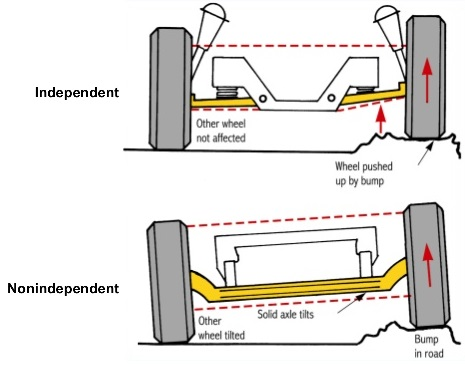
\includegraphics[width=9cm]{mech_ind_susp.jpg}
\end{center}
\caption{Advantage of independent over non-independent suspension.\cite{Dun_indsus}}
\label{fig:mech_indsus}
\end{figure}
\newline While non-independent suspension is mechanically simpler, it is easy to see from Figure \ref{fig:mech_indsus} that independent suspension has more benefits in terms of ride comfort, which in Tiberius' case is crucial to reduce the wear on its components. Thus it was decided that independent suspension was the preferred solution for the robot.
\newline
There are many ways of attaching the wheel of a vehicle to the chassis while allowing relative movement through a shock absorber. The most common method is to use wishbone linkages; these are Y-shaped links hinged on the chassis side, with a universal joint on the wheel side. A pair of wishbones attached at parallel points will allow the up-and-down motion of the wheel knuckle (dampened by a shock absorber) while keeping the wheel upright.
\begin{figure}[!htb]
\begin{center}
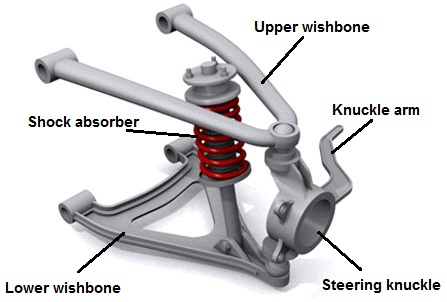
\includegraphics[width=8cm]{mech_double_wishbone.jpg}
\end{center}
\caption{Components of double-wishbone suspension.\cite{Dun_dbwb}}
\label{fig:mech_dbwb}
\end{figure}
\newline
Figure \ref{fig:mech_dbwb} shows the workings of a simple double-wishbone suspension unit. It is comprised of two wishbone linkages, a wheel knuckle which will hold the wheel shaft, and a shock absorber fixed to one of the wishbones. For wheels with steering systems, a control arm would be attached to the wheel knuckle.